% $Header: /Users/joseph/Documents/LaTeX/beamer/solutions/conference-talks/conference-ornate-20min.en.tex,v 90e850259b8b 2007/01/28 20:48:30 tantau $

\documentclass{beamer}

%\documentclass[handout]{beamer}

%\setbeameroption{show notes}

\usepackage{tikz}
\usepackage{xcolor}
\usepackage{tabu}
\usepackage{listings}
\usepackage{pifont}
\usepackage{todonotes}

\lstset{basicstyle=\ttfamily\scriptsize}
\lstset{escapeinside={(*}{*)}}

\definecolor{tableShade1}{gray}{0.92}
\definecolor{tableShade2}{gray}{0.97} 

% This file is a solution template for:

% - Talk at a conference/colloquium.
% - Talk length is about 20min.
% - Style is ornate.



% Copyright 2004 by Till Tantau <tantau@users.sourceforge.net>.
%
% In principle, this file can be redistributed and/or modified under
% the terms of the GNU Public License, version 2.
%
% However, this file is supposed to be a template to be modified
% for your own needs. For this reason, if you use this file as a
% template and not specifically distribute it as part of a another
% package/program, I grant the extra permission to freely copy and
% modify this file as you see fit and even to delete this copyright
% notice. 


\mode<presentation>
{
	\usepackage[icsa,logoseparator,nonav,slidecount,secheadingsfooter]{beamerthemeinformatics}
	% or ...
	
%	\setbeamercovered{transparent}
	% or whatever (possibly just delete it)
}

\setbeamercolor{alerted text}{fg=red}
\setbeamerfont{alerted text}{series=\bfseries}

\newcommand{\HWPlaceholder}[3]{
	\begin{figure}
	\begin{tikzpicture}
		\node[minimum height=#3, minimum width=#2,draw] at (0,0) {#1};
	\end{tikzpicture}
	\end{figure}
}

\usepackage[english]{babel}
% or whatever

\usepackage[latin1]{inputenc}
% or whatever

\usepackage{times}
\usepackage[T1]{fontenc}
% Or whatever. Note that the encoding and the font should match. If T1
% does not look nice, try deleting the line with the fontenc.

\title % (optional, use only with long paper titles)
{Building a GenSim Model}

\author % (optional, use only with lots of authors)
{Harry Wagstaff, Tom Spink, Bruno Bodin, Bjoern Franke}
% - Give the names in the same order as the appear in the paper.
% - Use the \inst{?} command only if the authors have different
%   affiliation.

\institute % (optional, but mostly needed)
{
	Institute for Computing Systems Architecture \\
	University of Edinburgh
}
% - Use the \inst command only if there are several affiliations.
% - Keep it simple, no one is interested in your street address.

\date % (optional, should be abbreviation of conference name)
{April 2018}
% - Either use conference name or its abbreviation.
% - Not really informative to the audience, more for people (including
%   yourself) who are reading the slides online

%\subject{Theoretical Computer Science}
% This is only inserted into the PDF information catalog. Can be left
% out. 



% If you have a file called "university-logo-filename.xxx", where xxx
% is a graphic format that can be processed by latex or pdflatex,
% resp., then you can add a logo as follows:

% \pgfdeclareimage[height=0.5cm]{university-logo}{university-logo-filename}
% \logo{\pgfuseimage{university-logo}}



% Delete this, if you do not want the table of contents to pop up at
% the beginning of each subsection:
%\AtBeginSubsection[]
%{
%	\begin{frame}<beamer>{Outline}
%		\tableofcontents[currentsection,currentsubsection]
%	\end{frame}
%}

% If you wish to uncover everything in a step-wise fashion, uncomment
% the following command: 

%\beamerdefaultoverlayspecification{<+->}

\begin{document}
	
\begin{frame}
  \titlepage
\end{frame}

% Structuring a talk is a difficult task and the following structure
% may not be suitable. Here are some rules that apply for this
% solution:
	
% - Exactly two or three sections (other than the summary).
% - At *most* three subsections per section.
% - Talk about 30s to 2min per frame. So there should be between about
% 15 and 30 frames, all told.
	
% - A conference audience is likely to know very little of what you
% are going to talk about. So *simplify*!
% - In a 20min talk, getting the main ideas across is hard
% enough. Leave out details, even if it means being less precise than
% you think necessary.
% - If you omit details that are vital to the proof/implementation,
% just say so once. Everybody will be happy with that.

\section{Introduction}
\subsection{Overview}
\begin{frame}{Introduction}

\end{frame}

\begin{frame}
	\tableofcontents
\end{frame}	



\begin{frame}{dummy}\end{frame}

\subsection{Existing Models}

\begin{frame}{Existing Models}

\end{frame}

\begin{frame}{ARMv7 Model}

\begin{itemize}
	\item Full ARM Core Instruction Set
	\item Thumb and Thumb-2 Support
	\item Some NEON and VFP Support
	\item User Mode and Full System (via Archsim)
\end{itemize}

\end{frame}

\begin{frame}{ARMv8 Model}

\begin{itemize}
	\item Full AArch64 Instruction Set
	\item Some FP and Vector Support
	\item Full-System Support (via Captive)
\end{itemize}

\end{frame}

\begin{frame}{RISC-V Model}

\begin{itemize}
	\item Full Core Instruction Set
	\item Some FP Support
	\item User Mode Only
\end{itemize}

\end{frame}


\section{System Description}
\subsection{}

\begin{frame}{Overview}

\end{frame}

\begin{frame}{Register File}
\end{frame}

\begin{frame}{Features}
\end{frame}

\begin{frame}{Instruction Sets}
\end{frame}

\subsection{Syntax Description}

\begin{frame}{Overview}

How are instructions encoded?

How do we decode them?

\end{frame}

\begin{frame}{GenSim Assumptions}

GenSim currently makes a few assumptions about instruction encoding:
\begin{itemize}
\item Instruction decoding is stateless
\item Instructions are standalone
\item Instructions execute in PC order
\end{itemize}

\end{frame}

\begin{frame}{GenSim Assumptions}

However, GenSim does have native support for the following features:
\begin{itemize}
\item Instruction Predication
\item Variable Length Instructions
\end{itemize}

\end{frame}


\begin{frame}{Formats}

Formats described using printf-like string
\begin{itemize}
\item Inspired by ArchC
\item Specify constant and variable fields
\end{itemize}

\end{frame}

\begin{frame}{Formats}

\centering
ARM Data-Processing (Register) Format

\includegraphics[width=\textwidth]{figures/format-arm}

\bigskip

PowerPC B-Form

\includegraphics[width=\textwidth]{figures/format-ppc}

\bigskip

RISC-V R-Type

\includegraphics[width=\textwidth]{figures/format-riscv}

\end{frame}

\begin{frame}[fragile]{Formats}

PowerPC B-Form


\includegraphics[width=\textwidth]{figures/format-ppc}

\begin{lstlisting}
"%opcd:6 %bo:5 %bi:5 %bd:14 %aa:1 %lk:1";
\end{lstlisting}

\bigskip

RISC-V R-Type


\includegraphics[width=\textwidth]{figures/format-riscv}

\begin{lstlisting}
"%funct7:7 %rs2:5 %rs1:5 %funct3:3 %rd:5 %opcode:7";
\end{lstlisting}

\end{frame}

\begin{frame}[fragile]{Formats}

\begin{lstlisting}

AC_ISA(riscv)
{

ac_format rtype = "%funct7:7 %rs2:5 %rs1:5 %funct3:3 %rd:5 %opcode:7";

}

\end{lstlisting}

\end{frame}

\begin{frame}{Instructions}

Instructions represent `individually decodable' units
\begin{itemize}
\item Somewhat flexible...
\item<2-> But decode as much as possible at decode time!
\item<3-> i.e., avoid general `ALU' instructions
\end{itemize}

\end{frame}

\begin{frame}[fragile]{Instructions}

\begin{lstlisting}

AC_ISA(riscv)
{

ac_format rtype = "%funct7:7 %rs2:5 %rs1:5 %funct3:3 %rd:5 %opcode:7";

ac_instr<rtype> add;

}

\end{lstlisting}
\end{frame}

\begin{frame}[fragile]{Decoding}

Let's consider an example from RISC-V:

\pause

\centering{
RISC-V R-Type

\includegraphics[width=\textwidth]{figures/format-riscv}
}

\bigskip
\pause

\centering{
RISC-V ADD
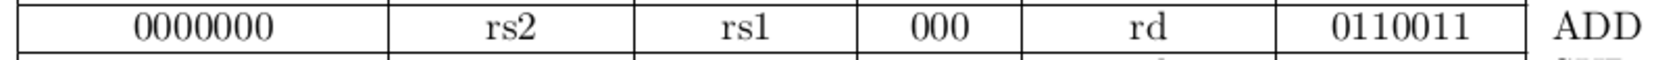
\includegraphics[width=\textwidth]{figures/risc-v-add}
}

\pause
\bigskip

\ttfamily\scriptsize{
\begin{tabular}{l l}
funct7 & 0b0000000 \\
funct3 & 0b000 \\
opcode & 0b0110011 \\
\end{tabular}
}

\pause

\begin{lstlisting}
add.set_decoder(funct7=0x0, funct=0x0, opcode=0x33);
\end{lstlisting}

\end{frame}

\begin{frame}[fragile]{Decoding}

\begin{lstlisting}

AC_ISA(riscv)
{

ac_format rtype = "%funct7:7 %rs2:5 %rs1:5 %funct3:3 %rd:5 %opcode:7";

ac_instr<rtype> add;

isa_ctor(riscv)
{

add.set_decoder(funct7=0x0, funct=0x0, opcode=0x33);

}

}

\end{lstlisting}
\end{frame}


\begin{frame}{Branch Metadata}

% DBT systems can take advantage

% Can't easily tell if an instruction is a jump
% - would need to detect writes to PC register
% - could be aliased with a bank

\end{frame}

\section{Semantics Description}
\subsection{}

\begin{frame}{dummy}\end{frame}

% Lots!


\section{Developing a Model}
\subsection{}

\begin{frame}{Developing a Model}
%Section title slide
\end{frame}

\begin{frame}{Developing a Model}

Model development is not too difficult but can take a long time

\begin{itemize}
\item ARMv7 and RISC-V models developed by students with no prior experience
\item Mostly a task of transcribing instruction pseudocode
\item Can be easy to introduce subtle errors or edge cases
\end{itemize}

\end{frame}

\begin{frame}{Our Workflow}
\end{frame}

\begin{frame}{Continuous Build}

% Jenkins
% Model tests

\end{frame}

\begin{frame}{Instruction Fuzzing}
Fuzzing is a randomized testing method

\begin{itemize}
\item<2-> Test instructions with many inputs against a ground truth
\item<3-> We use QEMU as a ground truth
\item<4-> \alert{Still problems with unspecified/undefined behaviour}
\end{itemize}


\onslide<5->{
We have our own tools for instruction fuzzing (which are linked from GenSim website)
}

\end{frame}

\begin{frame}{Debugging with Tracing}

Once we're confident that our model works, we can run some larger programs

\pause

But they might still go wrong! How do we debug this?

\end{frame}

\begin{frame}{Debugging with Tracing}

ArchSim can produce traces of architectural events
\begin{itemize}
\item Control flow/instructions executed
\item Register reads/writes
\item Memory reads/writes
\end{itemize}

\end{frame}

\begin{frame}{Debugging with Tracing}

\end{frame}

\begin{frame}{Model Optimisation}

Certain code structures can lead to poor performance:
\begin{itemize}
\item Very complex instructions
\item Non-fixed loop bounds
\item `Hand written' predicates
\item Enablement checks (can be solved using Features)
\end{itemize} 

\end{frame}

\begin{frame}[fragile]{Model Optimisation}
\begin{lstlisting}
if(read_register(FP_ENABLED)) {
	// do something
}
\end{lstlisting}

\begin{lstlisting}
if(__builtin_get_feature(FP_ENABLED)) {
	// do something
}
\end{lstlisting}

\end{frame}


\section{Conclusion}
\subsection{}

\begin{frame}{Recap}
To conclude:
\begin{itemize}
\item We've gone over the available models
\item Looked at the components of a model
\item I've shared some experiences building models
\item Briefly covered the internal flow of GenSim
\end{itemize}
\end{frame}

\begin{frame}{Conclusion}
	\centering
	Thanks for coming!
	
	\footnotesize{Any Questions?}
	
	\bigskip
	
	harry.wagstaff@gmail.com
	
	general@gensim.org
\end{frame}


\end{document}
